\documentclass[11pt]{article}
\usepackage{placeins}
\usepackage{graphicx}
\usepackage{url}

\begin{document}

\begin{titlepage}
	\begin{center}
    	
\includegraphics[scale=0.10]{du.png}\par
		\begin{Huge}
			\textsc{University of Dhaka}\par
		\end{Huge}
		\begin{Large}
			Department of Computer Science and Engineering\par \vspace{.5cm}
			CSE-3111 : Computer Networking Lab \\[12pt]	
			Lab Report 8:Implementation of Distance Vector Algorithm
		\end{Large}
	\end{center}  	
	\begin{large}
		\textbf{Submitted By:\\[12pt]}
			Name : Tasfia Tabassum\\[8pt]
			Roll No : 24\\[12pt]
			Name : Saima Akter\\[8pt]
			Roll No : 30\\[12pt]
		\textbf{Submitted On : \\[12pt]}
			April 6, 2023\\[20pt]
		\textbf{Submitted To :\\[12pt]}
			Dr. Md. Abdur Razzaque\\[12pt]
                Md Mahmudur Rahman\\[12pt]
                Md. Ashraful Islam\\[12pt]
                Md. Fahim Arefin
	\end{large}
\end{titlepage}

\section{Introduction}
The Distance Vector Algorithm (DVA) is a routing protocol used in computer networks to determine the best path for data to travel from one network node to another. Unlike the Link State Algorithm (LSA), which maintains a complete view of the network topology, the DVA works by exchanging routing information with neighboring nodes to determine the shortest path to a given destination. Each node maintains a routing table that contains information about the distance and next hop for each destination in the network. The DVA is relatively simple to implement and is well-suited for small to medium-sized networks, but it may not scale well to larger and more complex networks. Additionally, it can be slower to converge than the LSA, particularly in networks with frequent topology changes.

\subsection{Objectives}
\begin{itemize}
    \item Our objective is to understand and implement the Distance Vector Algorithm, simulate the algorithm's operation in a network topology and observe how routing tables are updated.

\end{itemize}
%%%%
%%%%
\section{Theory}
Distance Vector Algorithm is a type of routing algorithm used in computer networks to determine the optimal path for data transmission. It is based on the principle of sharing information between routers about the distance to other nodes in the network. Each router maintains a routing table that contains information about the distance to all nodes in the network and the next hop for each node. The distance is typically measured in terms of the number of hops required to reach the destination node.

The algorithm works by each router broadcasting its entire routing table to its neighboring routers. Each router then updates its own routing table based on the information received from its neighbors. This process is repeated periodically, allowing each router to gradually converge on the optimal path for each node in the network.

Distance Vector Algorithm has some drawbacks, such as slow convergence time and the potential for routing loops to occur. However, it is still widely used in small to medium-sized networks due to its simplicity and low resource requirements.

\section{Methodology}

\subsection{Router}

In the context of the Distance Vector Algorithm, a server refers to a network node that is responsible for maintaining and distributing information about the network topology to other nodes. The server is often referred to as a routing server, and it maintains a routing table that contains information about the distance and next hop to each node in the network.

The server periodically broadcasts its routing table to all other nodes in the network, and each node updates its own routing table based on the information received.

The server's primary role is to ensure that each node in the network has an up-to-date view of the network topology and can make informed decisions about routing packets. However, since each node in the network maintains its own routing table, the server does not have a complete view of the network topology like in the Link State Algorithm.

Despite its limitations, the Distance Vector Algorithm is a popular choice for smaller networks due to its simplicity and ease of implementation.


\subsection{Broadcaster}

In the context of the Distance Vector Algorithm (DVA), a broadcaster refers to a network node that is responsible for broadcasting its routing table to all neighboring nodes in the network. This broadcast includes information about the node's distance to other nodes in the network and the next hop to reach those nodes.

Each node in the network maintains a routing table that contains information about the shortest path to each destination in the network. The routing table is updated by exchanging routing information with neighboring nodes via broadcasts. When a node receives a broadcast from a neighboring node, it updates its own routing table accordingly.

The broadcaster's role is critical in the DVA, as it ensures that all nodes in the network have accurate and up-to-date routing information. Without the broadcaster, nodes would have to rely on periodic updates from each individual node in the network, which would be much less efficient.

However, the broadcaster can also be a source of issues in the DVA. For example, if a node broadcasts incorrect routing information, it can cause other nodes in the network to update their routing tables incorrectly, leading to suboptimal routing paths or routing loops. Therefore, it is important to ensure that broadcasters in the DVA are configured correctly and that appropriate mechanisms are in place to detect and correct routing errors.


\subsection{Receiver}

In the context of the Distance Vector Algorithm, a receiver refers to a network node that receives routing updates from neighboring nodes and updates its own routing table accordingly. The receiver continuously listens for routing updates and calculates the shortest path to each destination node based on the information received from neighboring nodes.

When a receiver receives a routing update from a neighboring node, it examines the update and determines whether it represents a better path to any of the destination nodes in its routing table. If the update represents a better path, the receiver updates its routing table accordingly.

If a receiver does not receive a routing update from a neighboring node within a certain amount of time, it assumes that the neighboring node is no longer reachable and marks the corresponding route as unreachable in its routing table. The receiver then broadcasts this information to its neighboring nodes, allowing them to update their own routing tables accordingly.

Overall, the receiver plays a critical role in the Distance Vector Algorithm by continuously updating its routing table based on the information received from neighboring nodes. This ensures that each node in the network has an up-to-date view of the network topology and can efficiently route packets to their destinations.



\subsection{Algorithm to implement distance vector algorithm : }
The graph we implemented using distance vector algorithm is given below:
 \begin{figure}[!h]
\centering
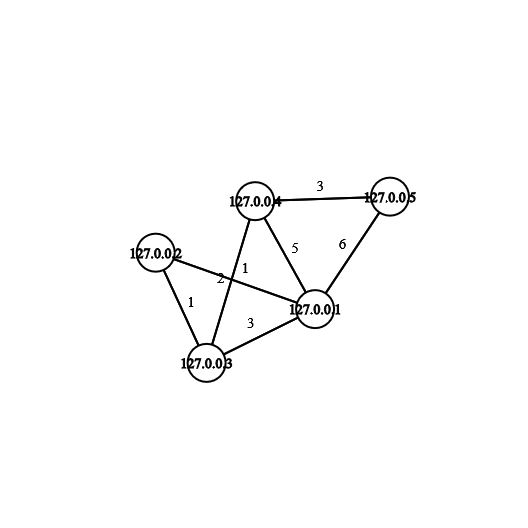
\includegraphics[width=\textwidth,height=10cm,keepaspectratio]{graph.png}
\caption{Graph Model of Routers}
\end{figure}
\FloatBarrier

\textbf{Routing Table of each Router within cost}\\[24pt]

Routing Table for '127.0.0.1' from the graph:\\[12pt] 
\begin{tabular}{ | m{8em} | m{5cm}| } 
  \hline
   127.0.0.1 & 0\\ 
  \hline
  127.0.0.2 & 1\\ 
  \hline
  127.0.0.3 & 3\\ 
  \hline
  127.0.0.4 & 5\\ 
  \hline
  127.0.0.5 & 6\\ 
  \hline
\end{tabular}\\[24pt]


Routing Table for '127.0.0.2' from the graph:\\[12pt] 
\begin{tabular}{ | m{8em} | m{5cm}| } 
    \hline
   127.0.0.2 & 0\\ 
  \hline
  127.0.0.1 & 1\\ 
  \hline
  127.0.0.3 & 1\\ 
  \hline
\end{tabular}\\[24pt]


Routing Table for '127.0.0.3' from the graph:\\[12pt] 
\begin{tabular}{ | m{8em} | m{5cm}| } 
    \hline
   127.0.0.3 & 0\\ 
  \hline
  127.0.0.1 & 3\\ 
  \hline
  127.0.0.2 & 1\\ 
  \hline
  127.0.0.4 & 2\\ 
  \hline
\end{tabular}\\[24pt]


Routing Table for '127.0.0.4' from the graph:\\[12pt] 
\begin{tabular}{ | m{8em} | m{5cm}| } 
    \hline
   127.0.0.4 & 0\\ 
  \hline
  127.0.0.1 & 5\\ 
  \hline
  127.0.0.3 & 2\\ 
  \hline
  127.0.0.5 & 3\\ 
  \hline
\end{tabular}\\[24pt]


Routing Table for '127.0.0.5' from the graph:\\[12pt]  
\begin{tabular}{ | m{8em} | m{5cm}| } 
    \hline
   127.0.0.5 & 0\\ 
  \hline
  127.0.0.1 & 6\\ 
  \hline
  127.0.0.4 & 3\\ 
  \hline
\end{tabular}\\[24pt]

\textbf{Step 1: }\\[12pt]
Initialize each node in the network with its distance to all other nodes. This distance can be represented as a vector of costs.


\textbf{Step 2: }\\[12pt]
Each node sends its distance vector to all of its neighboring nodes.

\textbf{Step 3: }\\[12pt]
When a node receives distance vectors from its neighbors, it updates its own distance vector based on the received vectors and its own cost to the neighbors.\\[12pt]

\textbf{Step 4: }\\[12pt]
After updating its distance vector, the node sends its new vector to all of its neighboring nodes.\\[12pt]

\textbf{Step 5: }\\[12pt]
Steps 3 and 4 are repeated until convergence is reached, meaning that no nodes update their distance vectors anymore.\\[12pt]

\textbf{Step 6: }\\[12pt]
To detect changes in the network topology, each node periodically sends its distance vector to its neighbors even if there are no updates.\\[12pt]

\textbf{Step 7: }\\[12pt]
If a node detects a change in the network, such as a link going down, it updates its distance vector and starts the convergence process again.\\[12pt]


\textbf{Method to  }\\[12pt]


\subsection{Screenshots output demonstrating the correct functionality of the program in various network scenarios: }

\textbf{Screenshots of router 1 : }\\[12pt]
 \begin{figure}[!h]
\centering
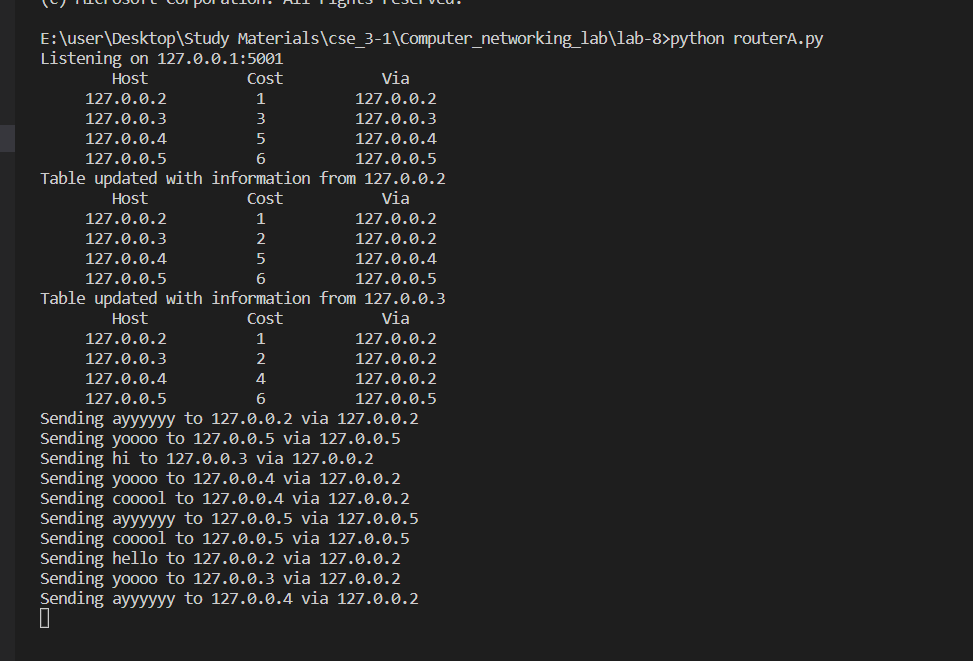
\includegraphics[width=\textwidth]{rA.png}
\caption{snapshot of Router 1}
\end{figure}
\FloatBarrier

\textbf{Screenshots of router 2 : }\\[12pt]
 \begin{figure}[!h]
\centering
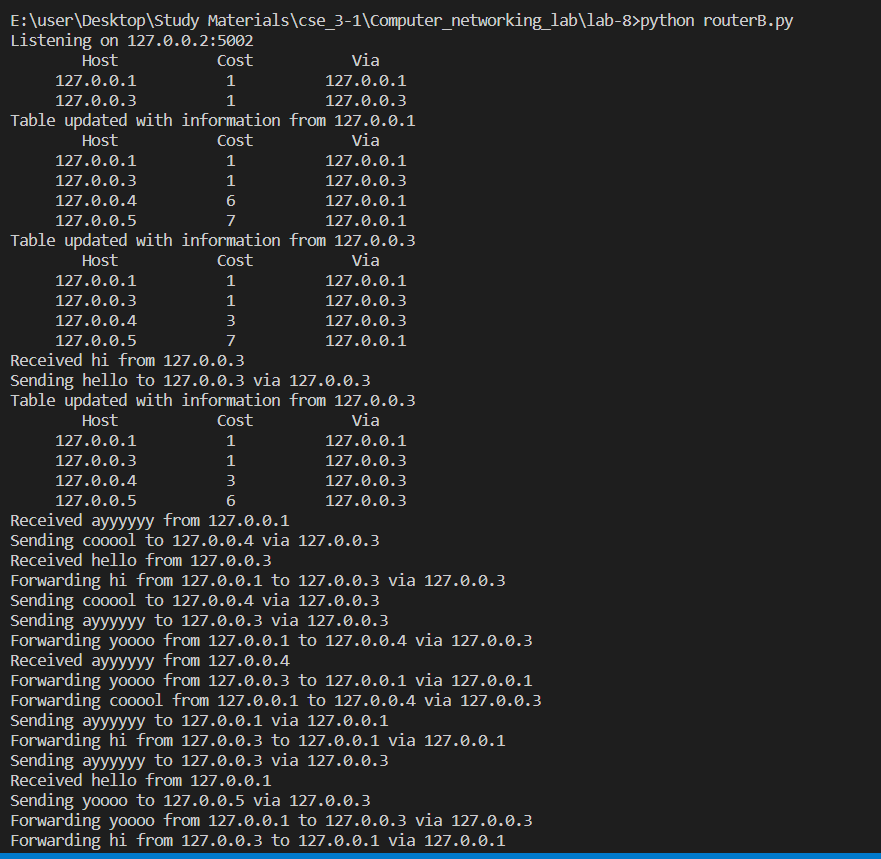
\includegraphics[width=\textwidth]{rB.png}
\caption{Snapshot of Router 2}
\end{figure}
\FloatBarrier

\textbf{Screenshots of router 3 : }\\[12pt]
 \begin{figure}[!h]
\centering
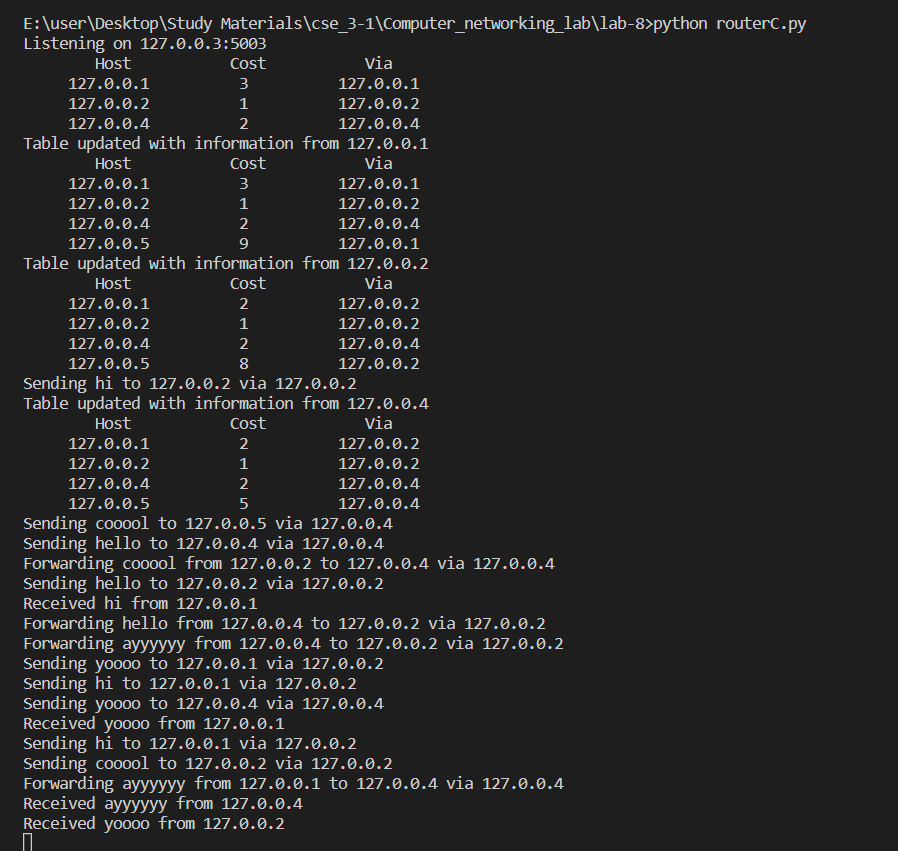
\includegraphics[width=\textwidth]{rC.png}
\caption{Snapshot of Router 3}
\end{figure}
\FloatBarrier

\textbf{Screenshots of router 4 : }\\[12pt]
 \begin{figure}[!h]
\centering
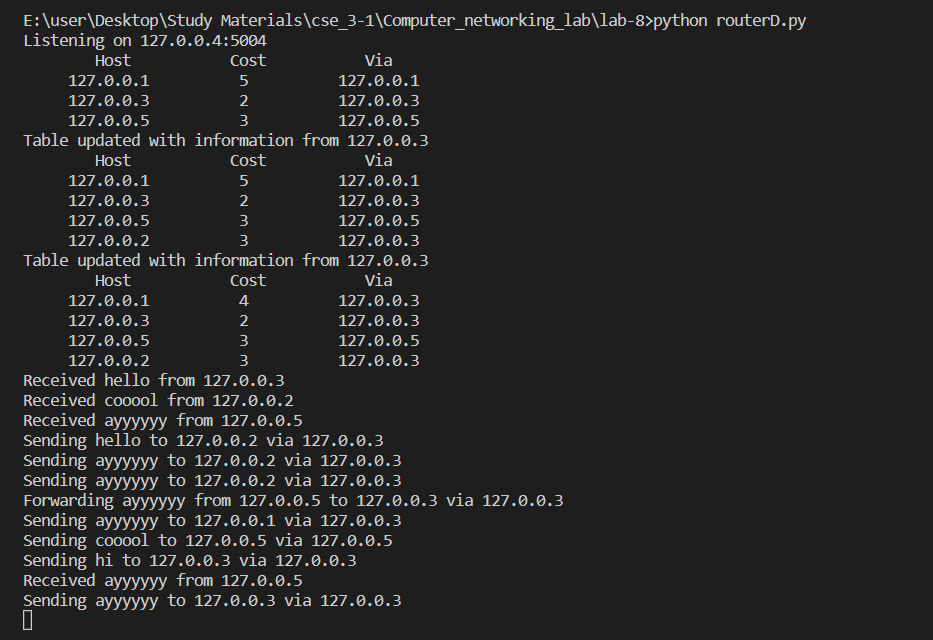
\includegraphics[width=\textwidth]{rD.png}
\caption{Snapshot of Router 4}
\end{figure}
\FloatBarrier

\textbf{Screenshots of router 5 : }\\[12pt]
 \begin{figure}[!h]
\centering
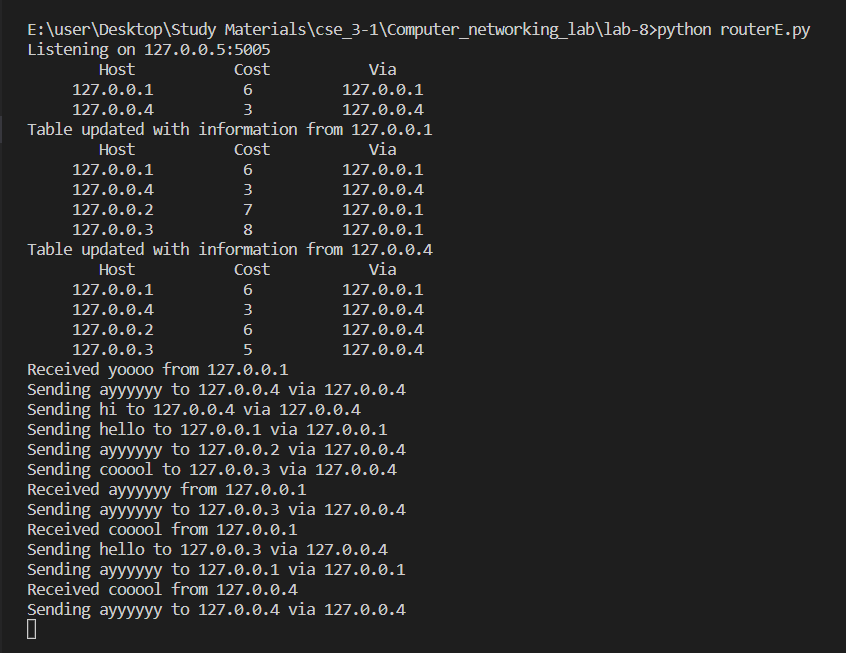
\includegraphics[width=\textwidth]{rE.png}
\caption{Snapshot of Router 5}
\end{figure}
\FloatBarrier


 \subsection{Comparison between Link state and Distance Vector algorithm}
 
Link state and distance vector algorithms are two popular routing algorithms used in computer networks. They both aim to find the best path to route data packets from the source to the destination.

One key difference between the two algorithms is the way they approach routing decisions. In the link state algorithm, each node in the network maintains a complete view of the network topology and calculates the shortest path to every other node using Dijkstra's algorithm. On the other hand, in the distance vector algorithm, each node only maintains information about its immediate neighbors and their distances to other nodes. The node updates its routing table by exchanging information with its neighbors.

Another difference is how they handle changes in the network topology. In the link state algorithm, each node detects changes in the network and broadcasts an update to all nodes in the network. In contrast, in the distance vector algorithm, each node periodically broadcasts its routing table to its neighbors, who in turn update their tables and broadcast them to their neighbors. This process continues until all nodes converge on the best routes.

The link state algorithm tends to have a higher overhead in terms of memory and processing power as it requires each node to maintain a complete view of the network topology. However, it offers faster convergence times and more reliable routing in large and complex networks. The distance vector algorithm, on the other hand, is simpler and less resource-intensive, making it suitable for smaller networks. However, it can suffer from issues such as slow convergence and the possibility of routing loops.


\section{Experience}
In the lab report on "Implementation of Distance Vector Algorithm" we conducted a comprehensive study on the implementation of distance vector algorithm. While working on the experiment, we faced challenges while implementing the bellman ford algorithm. At first we tried to implement bellman ford algorithm on the whole graph which led us to wrong answer. We solved this problem by taking distance vector of each router's neighbours' then calculating the minimum distance in bellman ford. 



\begin{thebibliography}{1}
\bibitem{book}  Computer networking : a top-down approach 6th ed.
\bibitem{StackOverflow} StackOverflow : \url{http://stackoverflow.com/}
\bibitem{Geeks for geeks} GeeksforGeeks : \url{https://www.geeksforgeeks.org/}
\end{thebibliography}

\end{document}